\documentclass{article}
\usepackage[utf8]{inputenc}
\usepackage[greek, brazil]{babel}
\usepackage[left=1cm, right=1.5cm, top=5cm, bottom=5cm]{geometry}
\usepackage{graphicx}
\usepackage{hyperref}
\usepackage[usenames,dvipsnames]{xcolor}
\renewcommand{\thefootnote}{\alph{footnote}}
\setlength{\parskip}{\baselineskip}
\setlength{\parindent}{0pt}
\hypersetup {
  colorlinks,
  citecolor = NavyBlue,
  filecolor = NavyBlue,
  linkcolor = NavyBlue,
  urlcolor = NavyBlue
}
\author{Lucas}
\title{Questões de Procedimentos, Restauração de Contexto, Salvamento de 
Contexto, etc.}
\begin{document}
\maketitle

% 112-118 pgs
\begin{enumerate}

\item Os passos para criação de procedimentos são:

  \begin{enumerate}
    \item Colocar os parâmetros em um lugar que o procedimentos possa acessar.

      \begin{verbatim}
        (param0, param1, param2, param3) -> ($a0, $a1, $a2, $a3)
      \end{verbatim}

    \item Transferir o fluxo de execução de instruções para o endereço do
    procedimento.

      \begin{verbatim}
        jal PROCEDIMENTO
      \end{verbatim}

    \item Adquirir espaço na pilha necessário para o procedimento e salvar o
    contexto.

      \begin{verbatim}
        addi $sp, $sp, -8  # 0x00000000 -> [[0][1][ 2][ 3]] \
        sw $s0, 0($sp)     # 0x00000004 -> [[4][5][ 6][ 7]]  |> dois espaços
        sw $s1, 4($sp)     # 0x00000008 -> [[8][9][10][11]] /
                                      |
                                      +--------------------> ponteiro setado
                                                             uma palavra à
                                                             frente
      \end{verbatim}

    \item Realizar a tarefa desejada.

      \begin{verbatim}
        sll $s0, $t1, 2
        addi $s0, $s0, 8
        lw $t2, 0($s0)
        andi $s1, $t2, 0x23
        ...
      \end{verbatim}

    \item Colocar o resultado em um lugar onde o programa chamador pode acessar.

      \begin{verbatim}
        move $v0, $s0
        move $v1, $s1
      \end{verbatim}

    \item Restaurar o contexto

      \begin{verbatim}
        lw $s1, 0($sp)
        lw $s0, 4($sp)
        addi $sp, $sp, 8
      \end{verbatim}

    \item Retornar o controle para o ponto de origem.

      \begin{verbatim}
        jr $ra
      \end{verbatim}

  \end{enumerate}

  \item Uma variável em C é geralmente uma localização na memória, e isso
  depende do tipo da variável e classe de armazenamento. Exemplos incluem
  inteiros e caracteres. C tem duas classes de armazenamento: \verb|automático|
  e \verb|estático|. Automático são locais para um procedimentos e são
  descartados quando o procedimento existe mais. Variáveis estáticas existem
  através \verb|saídas| de \verb|entradas| para procedimentos. Por fora de
  todos os outros procedimentos, variáveis em c são consideradas estáticas,
  como são qualquer tipo de variável declarada usando a palavra-chave
  \verb|estático|. O resto são considerados \verb|automático|. Para simplificar
  acesso para dados estáticos, software em MIPS reserva outros registradores
  chamado \verb|ponteiro global| ou  \$gp (Patterson Computer Org. and Design
  página 118, Hardware/Software Interface).

\end{enumerate}

\pagebreak
\begin{figure}[ht!]
  \centering
  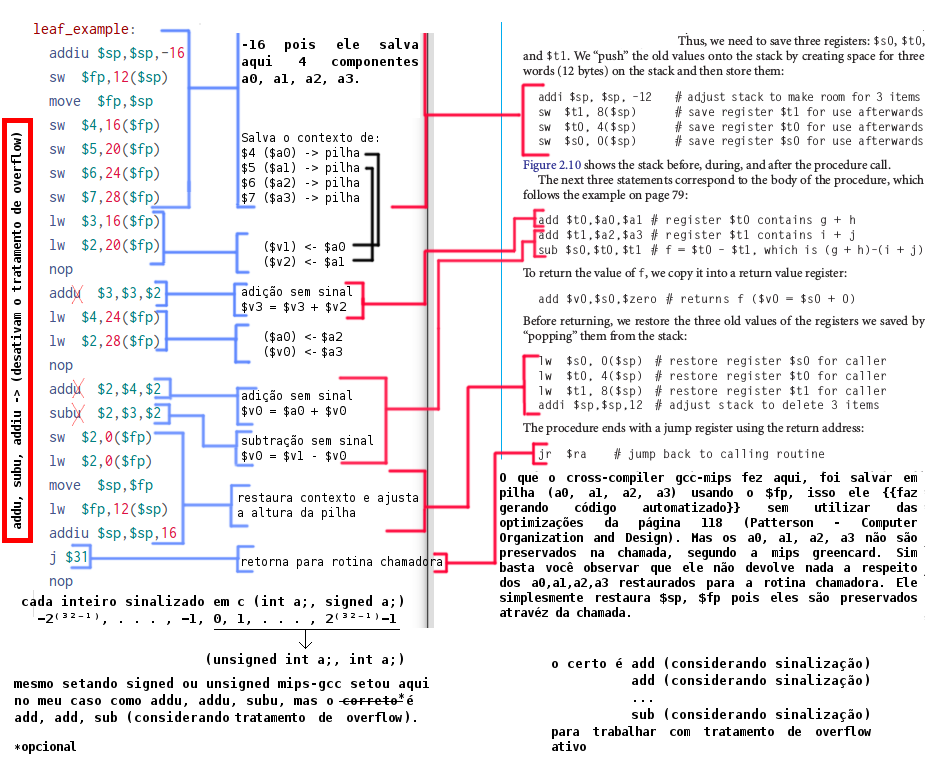
\includegraphics[width=\linewidth]{leaf_example.png}
  \caption{Addu, Subu, Addiu, desabilitam o tratamento de overflow, eles operam
  normalmente assim como as instruções Add, Sub, Addi, porém elas não tratam
  \underline{overflow}. Ao passo que Add, Sub, Addi, liberam para que o
  tratamento de overflow aconteça.}
\end{figure}

\pagebreak
Função Fatorial da Página 117, 118 David Patterson, Computer Organization and
Design.
\begin{verbatim}
fact:
  addiu  $sp,$sp,-24 # aqui o mips-gcc salva mais
  sw  $31,20($sp)    # do que o normal na página 117
  sw  $fp,16($sp)    # mas o mínimo que deve ser salvo
  move  $fp,$sp      # é $ra = $31 e também $4 = $a0
  sw  $4,24($fp)     # e também $a0 pois precisamos de
  lw  $2,24($fp)     # do rastro de n-1 n-2 n-3 que o
  nop                # fact deixa para trás (função recurssiva)
                     # você pode usar apenas o $sp se quiser

  bgtz  $2,$L2       # beq $2, $zero, L2
  nop                # se for mais que 0 vai para L2

  li  $2,1           # caso-contrario carrega o valor
  j  $L3             # 0x00000001 em $v0 para retornar
  nop                # e pula para L3

$L2:
  lw  $2,24($fp)     # $v0 <- $a0 (n>1 {2,3,4,5,....})
  nop                #
  addiu  $2,$2,-1    # $v0 -= 1 para colocar em fact()
  move  $4,$2        # pela convenção você envia por $a0
  jal  fact          # chama fact antes de multiplicar por * n
  nop                #

  move  $3,$2        # $v1 recebe $v0 (n antigo)
  lw  $2,24($fp)     # carrega $v0 (n novo) da chamada fact(n-1)
  nop                #
  mult  $3,$2        # multiplica n * fact (n - 1)
  mflo  $2           #
$L3:
  move  $sp,$fp      # caso n <= 1 por causa do if
  lw  $31,20($sp)    # dessa função recurssiva cairá
  lw  $fp,16($sp)    # aqui restaurara o necessário
  addiu  $sp,$sp,24  # e garantira que o $sp e $fp
  j  $31             # estarão preservados através
  nop                # de todas as chamadas de fact(n)
\end{verbatim}

Saiba que você pode eliminar o uso de \$fp e criar algumas optimizações, porém
esse código é o código gerado automaticamente por mipsel-none-elf-gcc é um
cross-compilador.


\clearpage

Converta o código em c abaixo para MIPS, lembrando os passos para criação de 
procedimentos genéricos. (a) salvar contexto (se necessário), (b) salvar \$ra, 
(c) dentro do escopo da rotina chamada -- criar alguma lógica, se necessária, 
de pré chamada de função aninhada, (d) passar parâmetros se existir função 
aninhada que requer parâmetros, (e) chamar usando \verb|jal| a rotina aninhada 
desejada mais os seus parâmetros usando \$a0, \$a1, \$a2, \$a3 ordenadamente e 
tantos quanto forem necessários (f) se necessário mais parâmetros então alocar 
em pilha, (g) pular definitivamente para função interna (g) para cada função 
chamada internar repetir c,d,e,f; (h) na volta de todas as funções mais 
internas restaurar o contexto, que foi salvo anteriormente, e continuar com a 
lógica do escopo, (i) observar possíveis labels, (j) observar possíveis branchs 
com lógica invertida, (l) lembrar de salvar o retorno das funções em 
registradores padrões i.e: \verb|$v0, $v1|, (m) lembrar de retornar utilizando 
\verb|jr $ra|\footnote{\textbf{Meu esquema para lembrar como criar os 
procedimentos genericamente, e seguindo o livro do Patterson \& Hennessy - 
Computer Organization and Design}}.

\begin{verbatim}
int alpha (int x, int y, int z) {
  if (x == 0) {
    return x + beta(z, y);
  } else {
    return x - beta(z, y);
  }
}

alpha: addi $sp, $sp, -8  ; abre locais na pilha para salvamento de contexto
       sw   $ra, 0($sp)   ; salva ra para o retorno final
       sw   $a0, 4($sp)   ; salva de x na pilha, pois é o único que eu p
                          ; precisarei usar depois do retorno de beta(z, y).
                          ; nesse exemplo, os valores que eu envio para beta
                          ; não irão ser usados depois do retorno de beta(z, y)
                          ; portanto eu não preciso salvar eles.
       add $a0, $a2, $0   ; a0 recebe o valor de z ($a2)
       add $a1, $a1, $0   ; a1 recebe o valor de y ($a1)
                          ; estou aqui ordenando e obedecendo o protótipo
                          ; da rotina beta(z, y)
       jal beta           ; salta para beta(z, y), suja ra, possívelmente
                          ; suja outros registradores i.e: a0, a1, a2....
       lw $a0, 4($sp)     ; restaura o contexto de a0
       lw $ra, 0($sp)     ; restaura o contexto de ra
       addi $sp, $sp, 8   ; fecha pilha
       bne $a0, $0, else  ; lógica do escopo da rotina alpha
       add $v0, $a0, $v0  ; v0 recebe a0 + beta(z,y)
       jr  $ra            ; retorna para a rotina chamadora
else:  sub $v0, $a0, $v0  ; v0 recebe a0 - beta(z,y)
       jr  $ra            ; retorna para a rotina chamadora
\end{verbatim}

\clearpage

\begin{verbatim}
int alpha (int x, int y, int z) {
  if (x == 0) {
    return x + beta(z - y);
  } else if (x == 1) {
    return x - beta(z - x);
  }
}
\end{verbatim}

Compilei o código acima para mips 32, {\bfseries você pode eliminar o uso de
\$fp se você preferir}. Além do mais você pode eliminar o uso da \textbf{LABEL}
\underline{L4}, e considerar redundante, colocando L1 onde aparecer L4. Para
máquina não é redundante, até então ela só traduz código, ela não acha que
existem coisas redundantes em relação a labels.

\begin{verbatim}
alpha:
  addiu $sp, $sp, -24  # abre espaço na pilha
  sw    $31, 20($sp)   # salva $ra
  sw    $fp, 16($sp)   # salva $fp
  move  $fp, $sp       # usa $fp como se fosse $sp
  sw    $4, 24($fp)    # salva a0     x     o compilador joga a[0-3] na pila
  sw    $5, 28($fp)    # salva a1     y     para poder usar eles com segurança
  sw    $6, 32($fp)    # salva a2     z     e não para preservar eles

  lw    $2, 24($fp)    # v0 recebe a0 (x) para testar no primeiro if
  nop
  bne   $2, $0, L2     # if $v0 != $zero pula para L2
  nop                  # lembrar que $v0 recebeu $a0
                       # eu sei que dá para eliminar esses
                       # passos intermediários, mas o compilador
                       # gera código automatizado
                       # caso-contrario pega $a2 (y)
                       # e também $a3 (z)
  lw    $3, 32($fp)    # v1 recebe a2 (z)
  lw    $2, 28($fp)    # v0 recebe a1 (y)
  nop
  subu  $2, $3, $2     # $v0 = $v0 - $v1, isto é calcular (z - y) para beta()
  move  $4, $2         # $a0 recebe $v0, para enviar à beta (convenção)
  jal   beta           # beta calcula usando $a0 que contém z - y e volta
  nop                  # a0 não vai ser preservado! através
                       # esse é um bom motivo para salvar $a0 no inicio
                       # da chamada, por isso se beta sujar a0
                       # então você perdeu a0 ...
  move  $3, $2         # $v1 recebe $v0
  lw    $2, 24($fp)    # $v0 recebe $a0 (que é x)
  nop
  addu  $2, $3, $2     # finalmente calcula x + beta(z - y)
  j     L1             # pula para L1 (que é a saída)
  nop

L2:
  lw    $3, 24($fp)    # pega o valor de $a0 salvado na pilha
  li    $2, 1          # carrega 0x1 em $2
  bne   $3, $2, L4     # caso x != 1 pula para L4

  lw    $3, 32($fp)    # carrega o valor de $a0 (z)
  lw    $2, 24($fp)    # carrega o valor de $a3 (x)
  nop
  subu  $2, $3, $2     # novamente mas agora é z - x
  move  $4, $2         # $a0 recebe $v0 com o resultado de z - x
  jal   beta           # pula para beta com a0 novo int beta(int);
  nop

  lw    $3, 24($fp)    # $v1 recebe $a0 (x salvo anteriormente,
  nop                  # pois beta não garante a0, a1, a2, ou a3)
  subu  $2, $3, $2     # finalmente faz x - beta(z - x)
  j     L1             # pula para L1 (que é a saída)
  nop

L4:
                       # L4 por sua vez não faz nada
                       # naturalmente ele caíra em L1
                       # L1 por sua vez é a saída do
                       # programa função int alpha(int x,int z,int y);
L1:
  move  $sp, $fp       # no livro do patterson ele simplifica o uso de $fp, $sp
  lw    $31, 20($sp)   # jogando toda a responsabilidade para $sp, mas o
  compilador
                       # restaura também o $ra para poder voltar ao chamador
                       # e também porque ele é garantidamente preservado
  lw    $fp, 16($sp)   # trabalha com $fp
  addiu $sp, $sp, 24   # veja que ele não preserva os $a0, $a1, $a2, $a3
  jr    $31            # volta para o chamador
  nop
\end{verbatim}

\pagebreak
\paragraph{2.19.1a}

A seguir todo o código traduzido para mips 32 da questão 2.19.1a da 4ª edição
\underline{revisada} do livro de organização e modulagem de computadores David
Patterson e John Hennessy página 197.

\begin{verbatim}
fib:
  # Memory Layout
  # [ 00 ] [ 01 ][ 02 ][ 03 ] -> espaço usado por fib: nesse exemplo
  # [ 04 ] [ 05 ][ 06 ][ 07 ] -> espaço usado por fib: nesse exemplo
  # [ 08 ] [ 09 ][ 10 ][ 11 ] -> espaço usado por fib: nesse exemplo
  # [ 12 ] [ 13 ][ 14 ][ 15 ] -> espaço usado por fib: nesse exemplo
  # [ 16 ] [ 17 ][ 18 ][ 19 ] -> espaço usado por fib: nesse exemplo
  # [ 20 ] [ 21 ][ 22 ][ 23 ] -> espaço usado por fib: nesse exemplo
  # [ 24 ] [ 25 ][ 26 ][ 27 ] -> espaço usado por fib: nesse exemplo
  # [ 28 ] [ 29 ][ 30 ][ 31 ] -> espaço usado por fib: nesse exemplo
  # [ 32 ] [ 33 ][ 34 ][ 35 ]

  addiu   $sp, $sp, -32 # abre espaço para salvar
  sw      $31, 28($sp)  # salva $ra para o retorno
  sw      $fp, 24($sp)  # salva $fp, poderia trabalhar apenas com $sp
  sw      $16, 20($sp)  # salva também $s0 == $16 (preservado através da
                        # chamada)
  move    $fp, $sp      # $fp recebe $sp (você poderia trabalhar apenas com $sp)
  sw      $4, 32($fp)   # salva $a0 em 32($fp)

  lw      $2, 32($fp)   # $v0 recebe $a0
  nop
  bne     $2, $0, L2    # se $a0 (em $v0) != $zero vai para L2 (onde tem outro
  teste)
  nop

  move    $2, $0        # carrega 0x0 para o primeiro retorno
  j       L3            # vai para L3 para restaurar contexto e retornar ao
  chamador
  nop

L2:

  lw      $3, 32($fp)   # carrega em $v0 o valor de $a0
  li      $2, 1         # carrega 1 em $v0
  bne     $3, $2, L4    # testa se $a0 (em $v0) se $v0 != 0x1 vai para L4
  nop

  li      $2, 1         # carrega 0x1 para o segundo retorno
  j       L3            # vai para L3 para restaurar contexto e retornar ao
  chamador
  nop

L4:
                        # aqui dentro temos a realização da chamada recursiva
  lw      $2, 32($fp)   # carrega $a0 em $v0
  nop
  addiu   $2, $2, -1    # faz n - 1 para a chamar fib(n-1)
  move    $4, $2        # move $v0 para $a0 (para enviar na chamada, convensão)
  jal     fib           # chamada recursivamente fib
  nop
                        # aqui temos o uso extra de $s0
                        # (que precisa ser restaurado ao final)
  move    $16, $2       # move $v0 para $s0
  lw      $2, 32($fp)   # carrega o valor de $a0 salvo no local 32($fp) em $v0
                        # a cada chamada recursiva a pilha vai abrindo novas
                        # 8 posições para novos dados, mas aqui pegamos sempre
                        # o n da vez para fazer corretamente fib(n-1) +
                        # fib(n-2);
  nop
  addiu   $2, $2, -2    # faz n - 2 para a chamar fib(n-2)
  move    $4, $2        # move $v0 para $a0 (para enviar na chamada, convensão)
  jal     fib           # chamada recursivamente fib
  nop

  addu    $2, $16, $2   # soma ambos fib(n-1) + fib(n-2)
                        # $v0 recebe $s0 + $v0 (v0 agora contém o resultado
                        # de fib(n-2)
L3:
  move    $sp, $fp
  lw      $31, 28($sp)  # restaura $ra
  lw      $fp, 24($sp)  # restaura $fp
  lw      $16, 20($sp)  # restaura $s0
  addiu   $sp, $sp, 32  # ajusta a pilha finalmente
  jr      $31           # retorna ao chamador
  nop

\end{verbatim}

\paragraph{2.19.2a}

A função recursiva com inline tem um certo limite que geralmente é imposto pelo
compilador, de por exemplo, entrar 8x dentro da recursão. Vou fazer o inline da
questão 2.19.1a da 4ª edição \underline{revisada} do livro de organização e
modulagem de computadores David Patterson e John Hennessy página 197. Para
realizar inline de funções recursivas você precisa primeira fazer um
esquemático da função recursiva em forma de árvore, vai abrindo as recursões
até um certo nível. Cada chamada irá requisitar novos registradores para
armazenar os valores.

\begin{verbatim}
int positive(int a, int b) {
  if (addit(a, b) > 0) {
    return 1;
  } else {
    return 0;
  }
}

int addit(int a, int b) {
  return a + b;
}
\end{verbatim}

Em MIPS 32 ficaria mais ou menos assim, primeiro sem inline:

\begin{verbatim}
positive:
  addiu  $sp, $sp, -24    # abre espaço na pilha
  sw  $31, 20($sp)        # salva ra
  sw  $fp, 16($sp)        # salva fp
  move  $fp, $sp          # fp recebe sp
  sw  $4, 24($fp)         # salva a0
  sw  $5, 28($fp)         # salva a1

  lw  $4, 24($fp)         # carrega a0
  lw  $5, 28($fp)         # carrega a1
  addu $2, $4, $5         # addit reduzido à uma instrução.
  nop                     # antes eram 14 instruções

  blez  $2, L2            # se o resultado em v0 (retornado por addit(a, b)
  nop                     # for menor ou igual zero então vai para L2

  li  $2, 1               # carrega 0x1 em $v0 por causa do return 1;
  j  $L3                  # pula para saida (ou melhor L3)
  nop

L2:
  move  $2, $0
L3:
  move  $sp, $fp          # sp recebe fp (dinovo, poderia ser usado apenas sp)
  lw  $31, 20($sp)        # restaura $ra
  lw  $fp, 16($sp)        # restura $fp
  addiu  $sp, $sp, 24     # restaura o ponteiro da pilha ("pop itens")
  jr  $31                 # volta para rotina chamadora
  nop
\end{verbatim}

Agora com inline em \underline{addit}. Com a adição de inline addit passou a
ser 1 instruções apenas dentro do corpo do procedimento positive, porém isso
tem um limite de até no máximo o uso de todos os registradores de uso geral no
MIPS 32, os registradores reservados seriam deixados privados.

\begin{verbatim}
positive:
  addiu  $sp, $sp, -24    # abre espaço na pilha
  sw  $31, 20($sp)        # salva ra
  sw  $fp, 16($sp)        # salva fp
  move  $fp, $sp          # fp recebe sp
  sw  $4, 24($fp)         # salva a0
  sw  $5, 28($fp)         # salva a1

  lw  $4, 24($fp)         # carrega a0
  lw  $5, 28($fp)         # carrega a1
  addu $2, $4, $5         # addit reduzido à uma instrução.
  nop                     # antes eram 14 instruções

  blez  $2, L2            # se o resultado em v0 (retornado por addit(a, b)
  nop                     # for menor ou igual zero então vai para L2

  li  $2, 1               # carrega 0x1 em $v0 por causa do return 1;
  j  $L3                  # pula para saida (ou melhor L3)
  nop

L2:
  move  $2, $0
L3:
  move  $sp, $fp          # sp recebe fp (dinovo, poderia ser usado apenas sp)
  lw  $31, 20($sp)        # restaura $ra
  lw  $fp, 16($sp)        # restura $fp
  addiu  $sp, $sp, 24     # restaura o ponteiro da pilha ("pop itens")
  jr  $31                 # volta para rotina chamadora
  nop
\end{verbatim}

\paragraph{2.19.4a}

Veja que eu não estou preservando a0, a1, a2, a3 pois as funções chamadas não
sou obrigadas, segundo a conversão de chamada, a preservarem eles. Porém dentro
da função elas podem preservar o necessário para executar a lógica desejada
pelo programador. O cross-compilador gcc-mips não altera a ordem lógica dos
parâmetros e isso é uma curiosidade, sendo que você não tem a \verb|func|
definida, nem mesmo seu protótipo. Ele mantém a ordem lógica dos parâmetros,
visando que alterar, reordenar a ordem lógica dos parâmetros para as funções
pode ser desastroso.

\begin{verbatim}
f:
  addiu  $sp, $sp, -0x14 # abre espaço na pilha
  sw     $31, 0x14 ($sp) # preserva o conteúdo de: ra
  sw     $4,  0x10 ($sp) # preserva o conteúdo de: a
  sw     $5,  0xC  ($sp) # preserva o conteúdo de: b
  sw     $6,  0x8  ($sp) # preserva o conteúdo de: c
  sw     $7,  0x4  ($sp) # preserva o conteúdo de: d

  lw  $4, 0x10 ($sp)     # carrega a0 com $a0
  lw  $5, 0xC  ($sp)     # carrega a1 com $a1
  jal func               # func mais interno func(a, b)
  nop

  move  $3, $2           # v1 recebe v0 (retorno do 1ro func(a,b))
  lw    $4, 0x8 ($sp)    # a0 recebe $a2 (int c, preservado na pilha)
  lw    $2, 0x4 ($sp)    # v0 recebe $a3 (int d, preservado na pilha)
  nop
  addu  $2, $4, $2       # v0 recebe c + d
  move  $4, $3           # mover $v1 para $a0 (primeiro parâmetro de func)
  move  $5, $2           # mover $v0 para $a1 (segundo parâmetro de func)
  jal   func             # salta para func novamente
  nop

  lw     $31, 0x14 ($sp) # restaura ra
  addiu  $sp, $sp, 0x14  # ajusta altura pilha
  jr     $31             # retorna a rotina chamadora
  nop
\end{verbatim}

\end{document}
